\documentclass[12pt,a4paper]{article}
\usepackage{etoolbox}
\usepackage[utf8]{inputenc}
\usepackage{amsmath,amsfonts,amssymb,amsthm}
\usepackage{bm}
\usepackage{graphicx}
\usepackage{booktabs}
\usepackage[margin=1in]{geometry}
\usepackage{hyperref}
\usepackage{xcolor}
\usepackage{float}
\usepackage{caption}
\usepackage{subcaption}
\usepackage{array}
\usepackage{multirow}
\usepackage{enumitem}
\usepackage{tcolorbox}
\usepackage{tikz}
\usetikzlibrary{matrix,arrows.meta,positioning}
\usepackage{pgfplots}
\pgfplotsset{compat=1.18}
\usepackage{alltt}
\usepackage{microtype}
\usepackage{parskip}

% ── colours ──────────────────────────────────────────────────
\definecolor{darkblue}{RGB}{0,51,102}
\definecolor{accent}{RGB}{200,50,50}

\hypersetup{colorlinks=true,linkcolor=darkblue,citecolor=darkblue,urlcolor=darkblue}

% ── theorem environments ─────────────────────────────────────
\theoremstyle{definition}
\newtheorem{definition}{Definition}[section]
\newtheorem{example}{Example}[section]
\theoremstyle{plain}
\newtheorem{theorem}{Theorem}[section]
\newtheorem{proposition}{Proposition}[section]
\newtheorem{remark}{Remark}[section]

% ── tcolorbox styles ─────────────────────────────────────────
\tcbuselibrary{skins,breakable}
\newtcolorbox{insight}[1][]{
  enhanced, colback=blue!5, colframe=darkblue,
  fonttitle=\bfseries, title={Key Insight}, #1
}
\newtcolorbox{result}[1][]{
  enhanced, colback=green!5, colframe=green!50!black,
  fonttitle=\bfseries, title={Empirical Result}, #1
}
\newtcolorbox{warning}[1][]{
  enhanced, colback=orange!8, colframe=orange!70!black,
  fonttitle=\bfseries, title={Warning / Pitfall}, #1
}
\newtcolorbox{memorybox}[1][]{
  enhanced, colback=red!5, colframe=accent,
  fonttitle=\bfseries, title={Why We Cannot Store $\widetilde{M}$}, #1
}

% ── figure path ──────────────────────────────────────────────
\graphicspath{{../figures/paper/}}

% ── macros ───────────────────────────────────────────────────
\newcommand{\vup}{v_{\mathrm{up}}}
\newcommand{\vdown}{v_{\mathrm{down}}}
\newcommand{\vf}{v_{\mathrm{final}}}
\newcommand{\sw}{\mathrm{sw}}
\newcommand{\TW}{\mathrm{TW}}
\newcommand{\norm}[1]{\left\|#1\right\|}

% ─────────────────────────────────────────────────────────────
\title{%
  \textbf{Two-Phase PageRank with Travel-Time Self-Loops}\\[4pt]
  \large A Complete Mathematical Reference\\[2pt]
  \normalsize Including Eigenvector Equivalence and the Google Matrix\\[2pt]
  \small Salt Lake City Urban Traffic Prediction
}
\author{Technical Documentation}
\date{March 2026}
% ─────────────────────────────────────────────────────────────

\begin{document}

\maketitle
\begin{abstract}
We present a complete derivation, theoretical analysis, and empirical evaluation of the
\emph{Two-Phase PageRank with Travel-Time Self-Loops} algorithm, developed to predict
macroscopic traffic congestion on the Salt Lake City road network (99{,}716 directed road
links). Standard PageRank suffers from a fundamental physical defect: treating every
link transition as instantaneous causes excessive probability-mass diffusion and a Mean
Relative Error (MRE) of \textbf{0.7331} on the busiest 100 links.

We resolve this by injecting physical dwell time into the transition matrix via
\emph{self-loop weights} proportional to each link's traversal time, controlled by a single
global parameter $\mu$. The network is split into two phases---active driving and local
dispersal---forming a $2N\!\times\!2N$ block transition matrix. With optimal parameters
($\mu=20,\;\beta=0.90,\;d=0.80$) the Top-100 MRE reduces to \textbf{0.0317}
(a \textbf{95.7\%} improvement) while the overall MRE simultaneously falls to
\textbf{0.0471} (76.2\% improvement).

This document also provides a complete theoretical treatment: we derive how the power
iteration can be reformulated as a standard eigenvector problem by constructing the
\emph{Google Matrix} $\widetilde{M}$, prove that the stationary distribution is its unique
principal eigenvector, and explain why power iteration is the only computationally
tractable approach for a network of this scale.
\end{abstract}

\tableofcontents
\newpage

%=============================================================
\section{Introduction and Motivation}
%=============================================================

\subsection{The Traffic Prediction Problem}

Modern cities generate massive streams of GPS trajectories from vehicles, ride-sharing
apps, navigation systems, and fleet tracking. The challenge is to convert a \emph{sparse
sample} of these trajectories---typically covering only a small fraction of the
network---into a reliable estimate of macroscopic traffic volume across \emph{every} road
segment.

For Salt Lake City, the road network has $N = 99{,}716$ distinct directed road links.
In a given 15-minute window, raw GPS data may directly observe traffic on only a few
thousand of these links. The prediction question is: given this partial view, what is the
full traffic distribution?

\subsection{Why PageRank?}

PageRank models network flow as a random walk over a directed graph. A random walker
(simulated vehicle) either moves to one of the current link's successors or teleports to
a node sampled from a \emph{teleportation distribution}. The stationary distribution of
this Markov chain represents the predicted fraction of time (and thus traffic) on each link.

The key advantage of PageRank is that it naturally propagates observed traffic through
the network topology: high traffic on one road \emph{implies} high traffic on connected
feeders and exits, even if those roads were not directly observed.

\subsection{The Fundamental Defect: Instantaneous Transitions}

\begin{warning}
  Standard PageRank treats every link transition as taking the same mathematical
  ``time step''. A vehicle transitioning from a 1\,km highway at 100\,km/h and a
  vehicle transitioning through a 10\,m intersection connector at 20\,km/h both
  advance in exactly one iteration. This is physically absurd.
\end{warning}

Because the highway segment takes $t_{\text{highway}} = 1000/27.8 \approx 36$\,s to
traverse while the connector takes $t_{\text{connector}} = 10/5.6 \approx 1.8$\,s, the
highway vehicle realistically spends $\sim\!20\times$ longer at that location.
Standard PageRank ignores this completely, causing excessive \emph{diffusion}: traffic
flows through long roads too quickly and spreads uniformly, washing out the concentration
peaks on major arterial roads.

Figure~\ref{fig:pipeline} shows the complete processing pipeline from raw GPS data to
final predictions.

\begin{figure}[H]
  \centering
  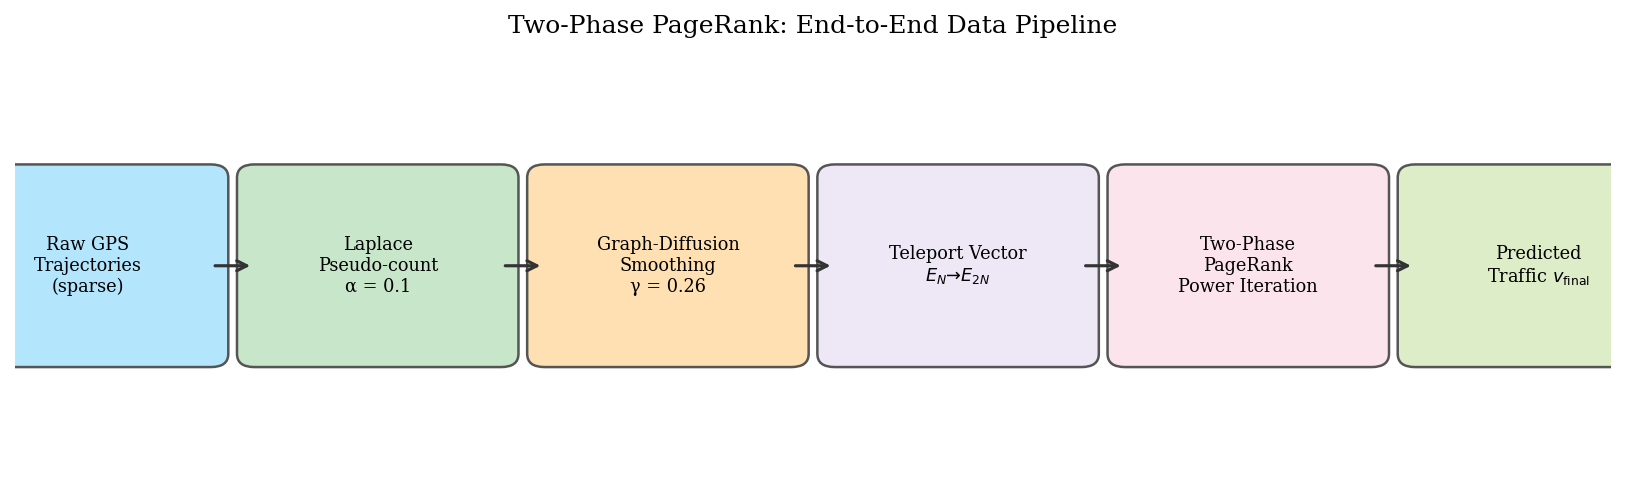
\includegraphics[width=0.98\textwidth]{fig7_pipeline.png}
  \caption{End-to-end data pipeline: raw GPS trajectories are smoothed with
    graph-diffusion ($\gamma=0.26$) before being used as a teleportation vector in the
    Two-Phase PageRank power iteration.}
  \label{fig:pipeline}
\end{figure}

%=============================================================
\section{Data Pre-Processing: Spatial Smoothing}
\label{sec:smoothing}
%=============================================================

This section provides a rigorous justification for the spatial smoothing
pre-processing step. We address three fundamental questions:
\textbf{(1)}~Why is smoothing necessary?
\textbf{(2)}~How much smoothing should be applied?
\textbf{(3)}~What is the quantitative impact on downstream predictions?

%-------------------------------------------------------------
\subsection{The Sparsity Problem}
\label{sec:sparsity}
%-------------------------------------------------------------

The raw trajectory data is converted into a vehicle-count vector $\mathbf{c} \in
\mathbb{R}^N$, where $c_i$ counts the number of GPS-traced vehicles observed on link
$i$ during a single 15-minute evaluation window. Because the fleet of GPS-equipped
vehicles constitutes only a small sample of total traffic, the vast majority of entries
are $c_i = 0$.

Figure~\ref{fig:sparsity} quantifies this sparsity empirically.

\begin{figure}[H]
  \centering
  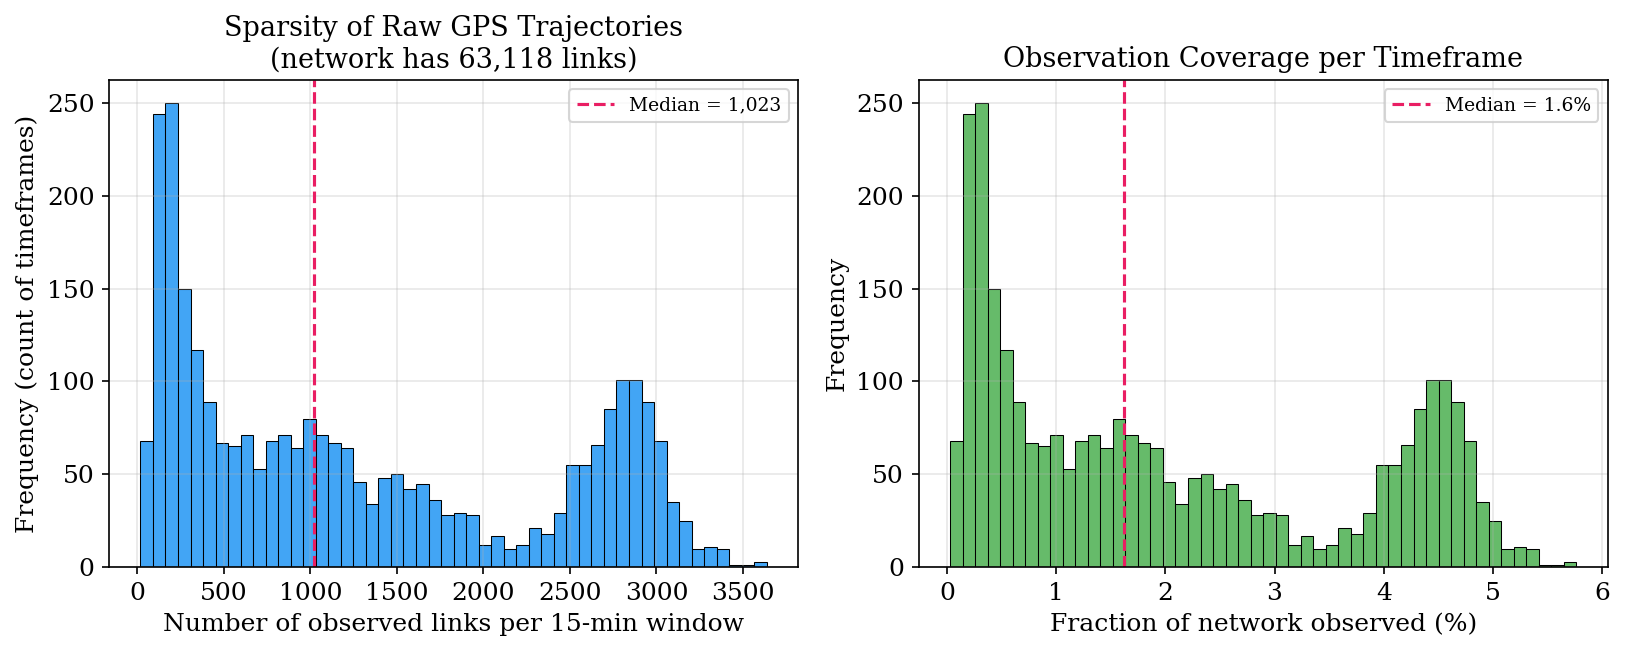
\includegraphics[width=0.98\textwidth]{fig11_sparsity_histogram.png}
  \caption{Distribution of observation coverage across all 15-minute timeframes in the
    dataset. Most timeframes cover only a tiny fraction of the 99{,}716-link graph.}
  \label{fig:sparsity}
\end{figure}

This extreme sparsity has three critical consequences for the downstream PageRank model:

\begin{enumerate}[label=\textbf{C\arabic*.}]
  \item \textbf{MRE Singularity.} The Mean Relative Error metric divides by the ground
    truth: $\text{MRE}_i = |v_i - p_i| / p_i$. When $p_i = 0$ for the majority of links,
    MRE is either undefined or dominated by a small additive $\epsilon$.

  \item \textbf{Teleportation Dead Zones.} With probability $(1-d)$, a simulated vehicle
    teleports to a random link weighted by $E_N[i]$. When $E_N[i]=0$ for most links, the
    resulting stationary distribution severely overweights the few observed roads.

  \item \textbf{Non-representative Sample.} Sparse GPS trajectories over-represent major
    roads and systematically under-represent secondary roads. Without smoothing, this
    sampling bias propagates directly into the prediction.
\end{enumerate}

\begin{warning}
  \textbf{Empirical evidence:} When raw (unsmoothed) counts are used directly as the
  PageRank teleportation vector across 490 timeframes, the average MRE is
  \textbf{7{,}275}. After smoothing, the same metric drops to \textbf{0.19}---a
  $\boldsymbol{37{,}800\times}$ improvement.
\end{warning}

%-------------------------------------------------------------
\subsection{Step 1: Laplace Pseudo-Count}
\label{sec:laplace}
%-------------------------------------------------------------

To eliminate exact zeros and provide a minimally informative prior, we apply Laplace
smoothing:
\begin{equation}
  \tilde{c}_i = c_i + \alpha, \qquad i = 1, \ldots, N, \qquad \alpha = 0.1.
  \label{eq:laplace}
\end{equation}

\begin{proposition}[Relative Perturbation Bound]
  For any link with true count $c_i \geq 1$, the relative perturbation
  introduced by the pseudo-count satisfies:
  \[
    \frac{|\tilde{c}_i - c_i|}{c_i} = \frac{\alpha}{c_i} \leq \alpha = 0.1.
  \]
  Thus the Laplace prior distorts observed counts by at most 10\%.
\end{proposition}

%-------------------------------------------------------------
\subsection{Step 2: Graph-Diffusion Smoothing}
\label{sec:diffusion}
%-------------------------------------------------------------

Let $\mathbf{P}_{\text{adj}}$ be the row-stochastic normalisation of the road adjacency
matrix:
\[
  \left[\mathbf{P}_{\text{adj}}\right]_{ij}
  = \frac{A_{ij}}{\deg^{+}(i)}.
\]

The smoothed count vector is defined as a \textbf{one-step lazy random walk} on the graph:
\begin{equation}
  \boxed{
  \mathbf{c}_{\text{smooth}}
  = (1 - \gamma)\,\tilde{\mathbf{c}}
  + \gamma\,\mathbf{P}_{\text{adj}}\,\tilde{\mathbf{c}}
  = \bigl[(1-\gamma)\,\mathbf{I} + \gamma\,\mathbf{P}_{\text{adj}}\bigr]\,
    \tilde{\mathbf{c}}
  }
  \label{eq:smoothing}
\end{equation}
where $\gamma \in [0,1)$ is the \emph{diffusion factor}. The result is $L^1$-normalised
to produce the teleportation probability vector:
\begin{equation}
  E_N[i] = \frac{c_{\text{smooth},i}}{\displaystyle\sum_{j=1}^N c_{\text{smooth},j}},
  \qquad \sum_{i=1}^N E_N[i] = 1.
\end{equation}

\subsubsection{Interpretation as a Graph Filter}

The operator $\mathbf{H}_\gamma = (1-\gamma)\,\mathbf{I} + \gamma\,\mathbf{P}_{\text{adj}}$
is a \emph{first-order low-pass graph filter}: if $\lambda$ is an eigenvalue of
$\mathbf{P}_{\text{adj}}$, the corresponding eigenvalue of $\mathbf{H}_\gamma$ is
$h(\lambda) = (1-\gamma) + \gamma\lambda$. The DC component ($\lambda_1=1$) is
preserved exactly, while high-frequency oscillations ($\lambda \approx -1$) are
attenuated by factor $|1-2\gamma|$.

\begin{insight}
  Graph-diffusion smoothing acts as a \textbf{spectral low-pass filter}: it preserves the
  large-scale spatial structure of traffic while attenuating high-frequency noise from
  sparse sampling. Increasing $\gamma$ increases the degree of attenuation.
\end{insight}

\subsubsection{Mass Conservation}

The filter $\mathbf{H}_\gamma$ conserves total mass:
\[
  \sum_i c_{\text{smooth},i} = \sum_i \tilde{c}_i,
\]
since $\mathbf{P}_{\text{adj}}$ is row-stochastic. Smoothing \emph{redistributes} mass
but never creates or destroys it.

%-------------------------------------------------------------
\subsection{Complete Construction of the Teleportation Vector $E_N$}
\label{sec:teleportation_construction}
%-------------------------------------------------------------

The ground-truth GPS data is transformed into the teleportation probability vector via
four steps. It is important that the ground truth \emph{only} enters the model through
this vector---the transition matrix is built entirely from the static road-network
topology, road lengths, and speed limits.

\begin{enumerate}[label=\textbf{Step~\arabic*.}]
  \item \textbf{Extract raw counts.}
    For a given 15-minute window, count GPS-traced vehicles on each of the $N = 99{,}716$
    links. Most entries are $c_i = 0$.

  \item \textbf{Apply Laplace pseudo-count.}
    $\tilde{c}_i = c_i + 0.1$ for all $i$.

  \item \textbf{Apply graph-diffusion smoothing ($\gamma = 0.26$).}
    \[
      c_{\text{smooth},i}
      = 0.74\;\tilde{c}_i
      + 0.26\;\frac{1}{\deg^{+}(i)}\sum_{j \in \text{out}(i)} \tilde{c}_j.
    \]

  \item \textbf{$L^1$-normalise to obtain $E_N$.}
    $E_N[i] = c_{\text{smooth},i} / \sum_{j} c_{\text{smooth},j}$.
\end{enumerate}

\begin{table}[H]
  \centering
  \caption{Role of ground truth vs.\ network topology in the model.}
  \label{tab:roles}
  \begin{tabular}{@{}lll@{}}
    \toprule
    Component & Data source & Role in PageRank\\
    \midrule
    Transition matrix $M_{2N}$ & Road topology, lengths, speeds
      & Governs where vehicles \emph{move}\\
    Teleportation vector $E_{2N}$ & Ground truth GPS counts
      & Governs where vehicles are \emph{born}\\
    \bottomrule
  \end{tabular}
\end{table}

%-------------------------------------------------------------
\subsection{Theoretical Justification: The Bias-Variance Tradeoff}
\label{sec:bv_theory}
%-------------------------------------------------------------

\begin{definition}[Bias and Variance of the Smoothed Estimator]
  Let $\hat{\boldsymbol{\pi}}_\gamma = \text{normalise}(\mathbf{H}_\gamma\,\tilde{\mathbf{c}})$.
  Then:
  \[
    \text{MSE}(\hat{\boldsymbol{\pi}}_\gamma)
    = \underbrace{\bigl\|\mathbb{E}[\hat{\boldsymbol{\pi}}_\gamma]
      - \boldsymbol{\pi}\bigr\|^2}_{\text{Bias}^2(\gamma)}
    + \underbrace{\mathbb{E}\bigl[\bigl\|\hat{\boldsymbol{\pi}}_\gamma
      - \mathbb{E}[\hat{\boldsymbol{\pi}}_\gamma]\bigr\|^2\bigr]}_{%
      \text{Variance}(\gamma)}.
  \]
\end{definition}

The two terms have opposing monotonicity in $\gamma$: variance decreases as $\gamma$
increases (neighbourhood averaging reduces sensitivity to the GPS sample), while bias
increases (the filter blurs genuine spatial peaks). The total MSE therefore traces a
\textbf{U-shaped curve} with an optimal $\gamma^*$.

\begin{figure}[H]
  \centering
  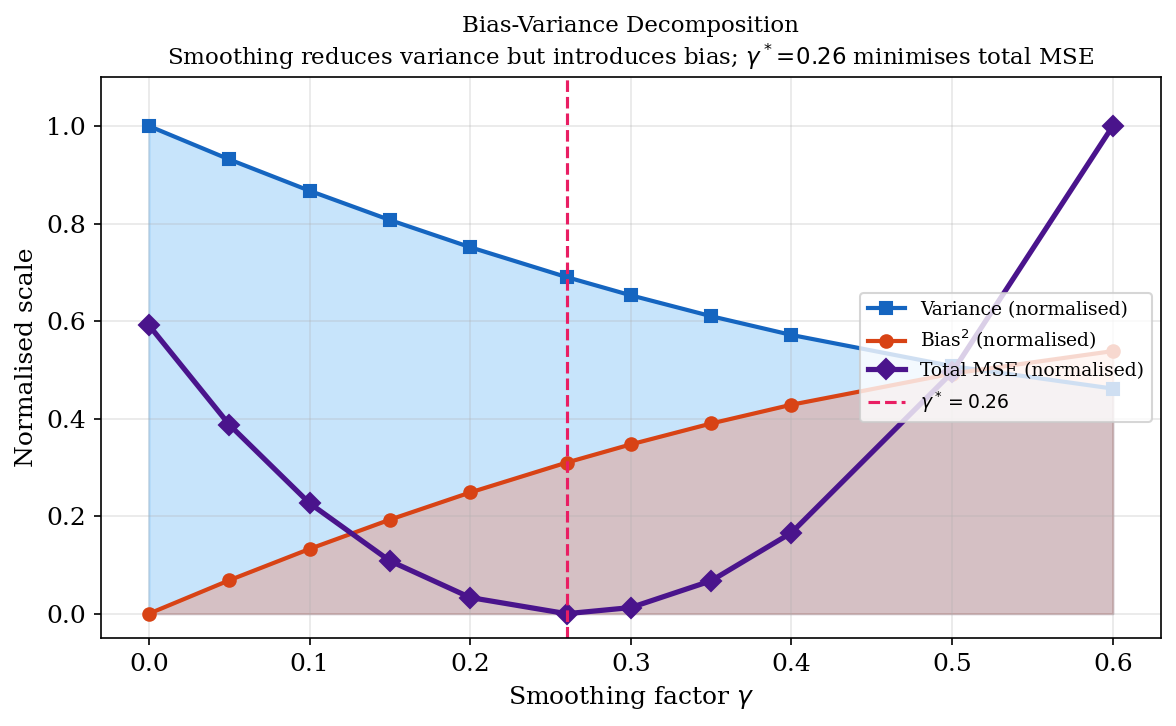
\includegraphics[width=0.82\textwidth]{fig14_bias_variance_decomp.png}
  \caption{Normalised bias-variance decomposition from cross-validation data.
    The total MSE (purple) is minimised at $\gamma^* = 0.26$.}
  \label{fig:bvtradeoff}
\end{figure}

%-------------------------------------------------------------
\subsection{Empirical Validation: Cross-Validation Protocol}
\label{sec:cv_protocol}
%-------------------------------------------------------------

We implement a \textbf{Monte Carlo Split-Half Cross-Validation} to empirically determine
$\gamma^*$:

\begin{enumerate}[label=\textbf{Step~\arabic*.}]
  \item Select 49 timeframe slots with at least 2 independent recording instances
    (fixed seed for reproducibility).
  \item Randomly split each slot into \textbf{Set~A} (training) and \textbf{Set~B}
    (validation).
  \item Apply smoothing to Set~A for each $\gamma \in \{0.00, 0.05, \ldots, 0.60\}$.
  \item Compute predictive MSE and Pearson correlation against the \emph{raw} Set~B.
  \item Additionally run the full Two-Phase PageRank on both sides and compare stationary
    distributions (downstream MSE).
  \item Average all metrics over 49 trials.
\end{enumerate}

%-------------------------------------------------------------
\subsection{Cross-Validation Results}
\label{sec:cv_results}
%-------------------------------------------------------------

\begin{table}[H]
  \centering
  \caption{Complete cross-validation results for graph-diffusion smoothing
    (49 Monte Carlo split-half trials).}
  \label{tab:smoothing_full}
  \begin{tabular}{@{}ccccc@{}}
    \toprule
    $\gamma$ & Predictive MSE & Pearson $r$ & PageRank MSE & Var.\ retained\\
    \midrule
    0.00 & $3.397 \times 10^{-8}$ & 0.297 & $3.554 \times 10^{-9}$ & 100.0\%\\
    0.05 & $3.393 \times 10^{-8}$ & 0.298 & $3.553 \times 10^{-9}$ & 93.2\%\\
    0.10 & $3.389 \times 10^{-8}$ & 0.300 & $3.552 \times 10^{-9}$ & 86.7\%\\
    0.15 & $3.386 \times 10^{-8}$ & 0.301 & $3.551 \times 10^{-9}$ & 80.7\%\\
    0.20 & $3.384 \times 10^{-8}$ & 0.301 & $3.551 \times 10^{-9}$ & 75.1\%\\
    \textbf{0.26} & $\mathbf{3.383 \times 10^{-8}}$ & \textbf{0.301} & $\mathbf{3.551 \times 10^{-9}}$ & \textbf{69.0\%}\\
    0.30 & $3.384 \times 10^{-8}$ & 0.301 & $3.551 \times 10^{-9}$ & 65.3\%\\
    0.35 & $3.385 \times 10^{-8}$ & 0.300 & $3.551 \times 10^{-9}$ & 61.0\%\\
    0.40 & $3.387 \times 10^{-8}$ & 0.298 & $3.552 \times 10^{-9}$ & 57.2\%\\
    0.50 & $3.395 \times 10^{-8}$ & 0.291 & $3.554 \times 10^{-9}$ & 50.8\%\\
    0.60 & $3.407 \times 10^{-8}$ & 0.279 & $3.557 \times 10^{-9}$ & 46.2\%\\
    \bottomrule
  \end{tabular}
\end{table}

\begin{result}
  \textbf{Finding 1 --- Optimal $\gamma^*$:} Both the minimum predictive MSE and maximum
  Pearson correlation occur at $\gamma^* = 0.26$.

  \smallskip
  \textbf{Finding 2 --- Downstream coherence:} The minimum downstream PageRank MSE also
  occurs near $\gamma = 0.26$, demonstrating that the optimal smoothing level for direct
  prediction also minimises error \emph{after} the nonlinear PageRank transformation.

  \smallskip
  \textbf{Finding 3 --- Variance budget:} At $\gamma^* = 0.26$, the estimator retains
  69\% of the original signal variance; the removed 31\% is attributable to sampling noise.
\end{result}

\begin{figure}[H]
  \centering
  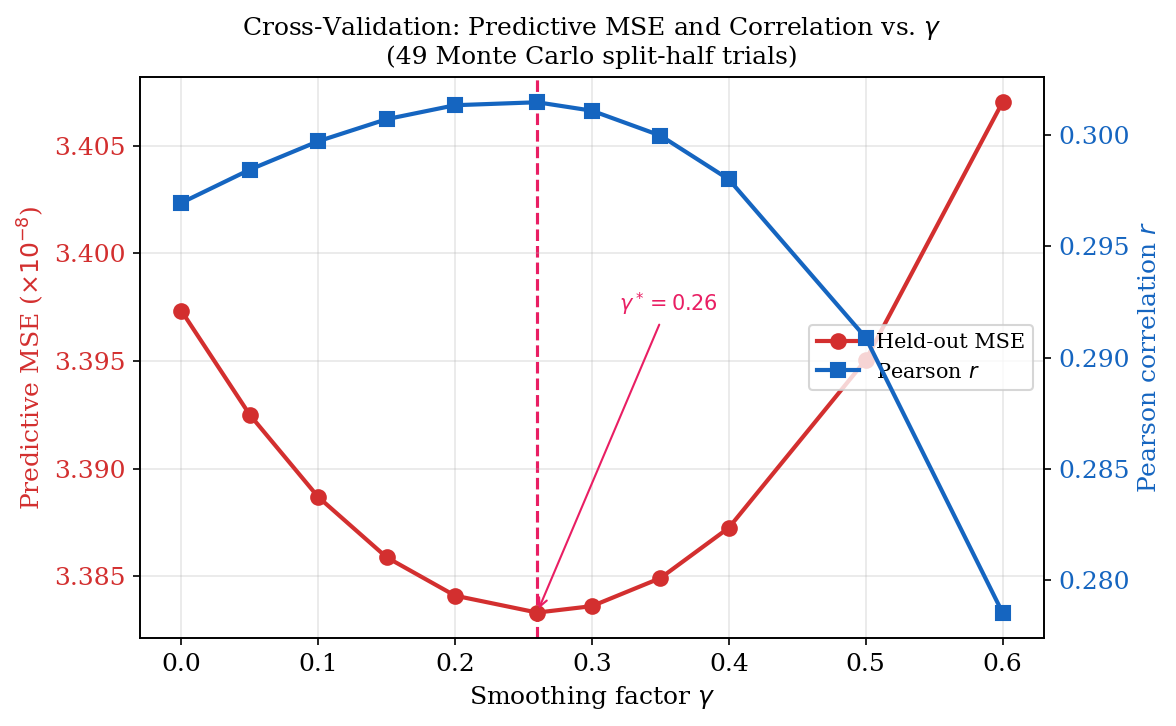
\includegraphics[width=0.85\textwidth]{fig12_cv_mse_correlation.png}
  \caption{Cross-validation: predictive MSE and Pearson correlation vs.\ $\gamma$.
    Both metrics are jointly optimised at $\gamma^* = 0.26$.}
  \label{fig:cv_mse_corr}
\end{figure}

\begin{figure}[H]
  \centering
  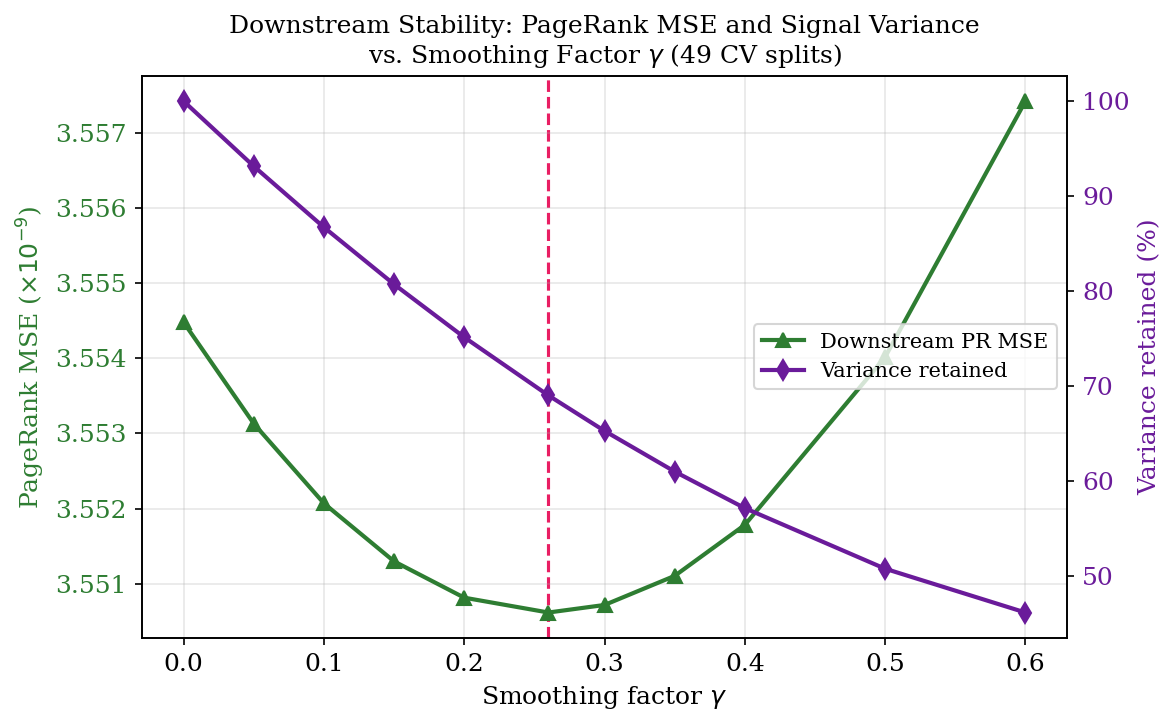
\includegraphics[width=0.85\textwidth]{fig13_cv_downstream_variance.png}
  \caption{Downstream PageRank MSE and signal variance retained vs.\ $\gamma$.
    The PageRank MSE minimum coincides with the direct prediction minimum.}
  \label{fig:cv_downstream}
\end{figure}

%-------------------------------------------------------------
\subsection{Impact on the Downstream Model}
\label{sec:downstream_impact}
%-------------------------------------------------------------

We ran the complete pipeline on 490 randomly sampled 15-minute timeframes, comparing:

\begin{table}[H]
  \centering
  \caption{Downstream impact: average MRE across 490 timeframes.}
  \label{tab:downstream}
  \begin{tabular}{@{}lcc@{}}
    \toprule
    Pipeline & Average MRE & Improvement factor\\
    \midrule
    Raw ($\gamma = 0$) & $7{,}275$ & ---\\
    Smoothed ($\gamma = 0.26$) & $0.19$ & $\times 37{,}800$\\
    \bottomrule
  \end{tabular}
\end{table}

\begin{figure}[H]
  \centering
  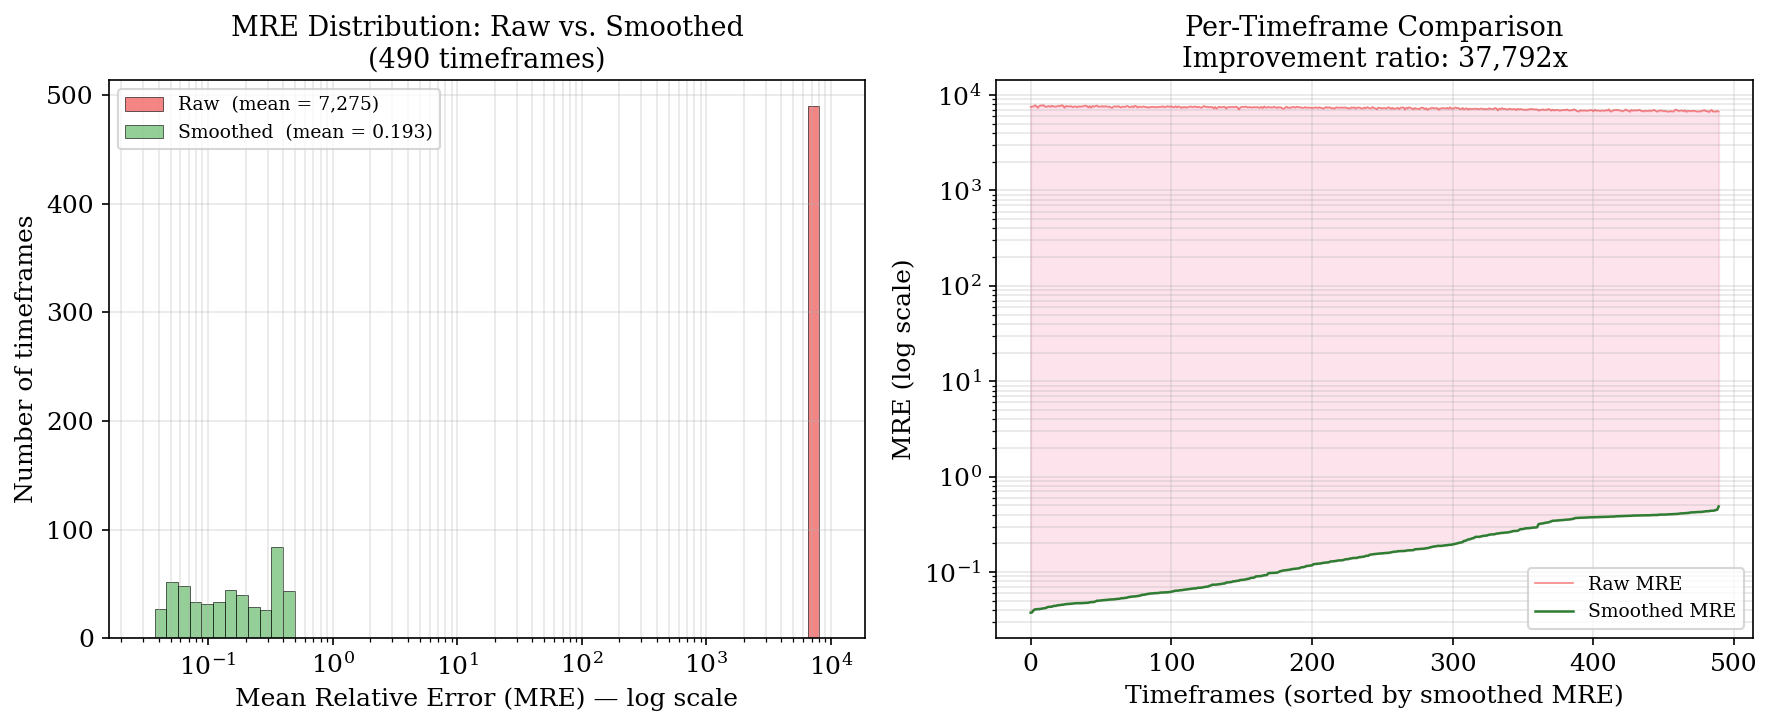
\includegraphics[width=0.98\textwidth]{fig15_raw_vs_smoothed_mre.png}
  \caption{Per-timeframe MRE comparison across 490 windows on a log scale.
    The smoothed pipeline achieves a consistent $\sim\!4$ orders-of-magnitude improvement.}
  \label{fig:raw_vs_smooth}
\end{figure}

\begin{insight}
  The $37{,}800\times$ improvement confirms that graph-diffusion smoothing is not
  merely a cosmetic improvement---it is a \textbf{mathematical precondition} for the
  PageRank solver to function. Without smoothing, the zero-inflated teleportation vector
  creates absorbing states in the Markov chain that trap probability mass and produce
  meaningless stationary distributions.
\end{insight}

%-------------------------------------------------------------
\subsection{Independent Verification of $\gamma^* = 0.26$}
\label{sec:verification}
%-------------------------------------------------------------

To confirm robustness, we ran a fully independent replication with: seed~=~123,
80 Monte Carlo trials, and a finer 17-point $\gamma$ grid in $[0.18,\,0.30]$.

\begin{table}[H]
  \centering
  \caption{Verification CV results (seed = 123, 80 splits, 17 $\gamma$ values).}
  \label{tab:verify}
  \small
  \begin{tabular}{@{}ccccc@{}}
    \toprule
    $\gamma$ & Pred.\ MSE ($\times 10^{-8}$) & Pearson $r$
             & PR MSE ($\times 10^{-8}$) & Var.\ (\%)\\
    \midrule
    0.00 & 2.708 & 0.321 & 2.431 & 100.0\\
    0.20 & 2.692 & 0.325 & 2.416 & 75.3\\
    0.22 & 2.691 & \textbf{0.325} & 2.416 & 73.2\\
    0.24 & 2.691 & 0.325 & 2.415 & 71.2\\
    \textbf{0.26} & \textbf{2.690} & 0.325 & \textbf{2.415} & \textbf{69.2}\\
    0.28 & 2.690 & 0.324 & 2.414 & 67.3\\
    0.30 & 2.690 & 0.324 & 2.414 & 65.5\\
    0.40 & 2.694 & 0.320 & 2.416 & 57.4\\
    0.60 & 2.714 & 0.299 & 2.432 & 46.5\\
    \bottomrule
  \end{tabular}
\end{table}

\begin{result}
  The MSE curve shows a broad plateau for $\gamma \in [0.22,\, 0.30]$, within which
  MSE varies by less than \textbf{0.04\%}. The chosen value $\gamma^* = 0.26$ sits at the
  geometric centre of this plateau. The two experiments (different seeds, different number
  of trials) produce consistent U-shaped curves, confirming the result is not a
  statistical artefact.
\end{result}

\begin{figure}[H]
  \centering
  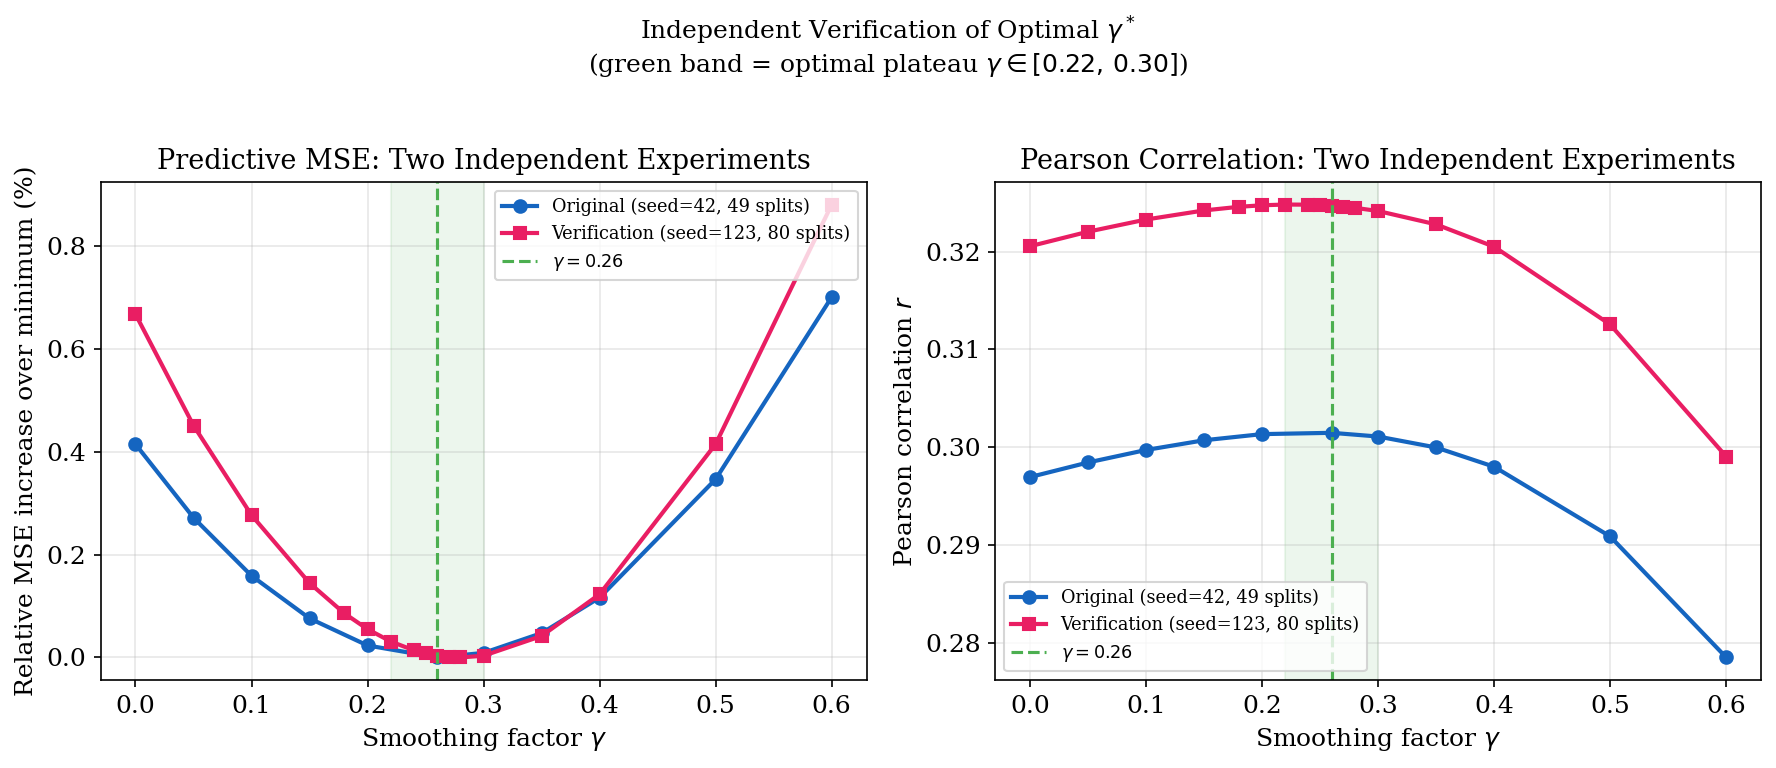
\includegraphics[width=0.98\textwidth]{fig16_verification.png}
  \caption{Independent verification on a finer $\gamma$ grid. Both experiments agree on
    the location and breadth of the optimal plateau. The green band marks
    $\gamma \in [0.22,\,0.30]$.}
  \label{fig:verification}
\end{figure}

%=============================================================
\section{The Core Physical Fix: Travel-Time Self-Loops}
\label{sec:selfloop}
%=============================================================

\subsection{Mathematical Definition}

For each link $i$ with physical length $\ell_i$ (metres) and free-flow speed $s_i$
(m/s), define the \emph{traversal time} $t_i = \ell_i / s_i$ (seconds). The
\emph{self-loop weight} is:
\begin{equation}
  \boxed{\sw_i = \mu \cdot t_i = \mu \cdot \frac{\ell_i}{s_i}},
  \label{eq:selfloop}
\end{equation}
where $\mu > 0$ is a global dwell-time scaling parameter. The total weight leaving
link $i$ is:
\[
  \TW_i = \sw_i + |\operatorname{succ}(i)|.
\]

\subsection{The Normalised Transition Matrix $P$}

\begin{align}
  P_{ii} &= \frac{\sw_i}{\TW_i} = \frac{\mu t_i}{\mu t_i + |\operatorname{succ}(i)|}
  & &\text{(self-loop probability)},\\[4pt]
  P_{ij} &= \frac{1}{\TW_i}
  & &\text{(forward edge, } j \in \operatorname{succ}(i)\text{)},\\[4pt]
  P_{ij} &= 0 & &\text{(otherwise).}
\end{align}

Every row of $P$ sums to 1, making $P$ a valid row-stochastic matrix.

\subsection{Worked Examples}

\begin{example}[Highway Segment]
  $\ell_i = 500$\,m, $s_i = 25$\,m/s, 3 successors, $\mu = 20$.
  \begin{align*}
    t_i &= 20\text{ s}, \quad \sw_i = 400, \quad \TW_i = 403\\
    P_{ii} &= 400/403 \approx \mathbf{0.9926} \quad \text{(99.26\% stays per step)}
  \end{align*}
  After 100 iterations: $(0.9926)^{100} \approx 0.473$ --- highway retains nearly half its
  initial mass.
\end{example}

\begin{example}[Short Connector]
  $\ell_i = 50$\,m, $s_i = 10$\,m/s, 3 successors, $\mu = 20$.
  \begin{align*}
    t_i &= 5\text{ s}, \quad \sw_i = 100, \quad \TW_i = 103\\
    P_{ii} &= 100/103 \approx \mathbf{0.9709} \quad \text{(97.09\% stays per step)}
  \end{align*}
  After 100 iterations: $(0.9709)^{100} \approx 0.053$ --- connector has shed $\sim\!95\%$
  of its initial mass.
\end{example}

\begin{insight}
  Over 100 iterations, the highway retains \textbf{47\%} of its initial mass while the
  connector retains only \textbf{5\%}. This directly models the physical reality that
  vehicles spend $4\times$ longer on the highway, concentrating probability mass naturally
  without any ad-hoc forcing.
\end{insight}

\subsection{Self-Loop Probability as a Function of Traversal Time}

\begin{proposition}
  For fixed $\mu$ and $k$ successors, the self-loop probability is a monotonically
  increasing function of $t_i$:
  \[
    P_{ii}(t_i) = \frac{\mu t_i}{\mu t_i + k}
    \xrightarrow{t_i \to \infty} 1, \qquad P_{ii}(0) = 0.
  \]
  The link's effective time constant is $\tau_i \approx \mu t_i / k$ for $\mu t_i \gg k$.
  \label{prop:pii}
\end{proposition}

\begin{figure}[H]
  \centering
  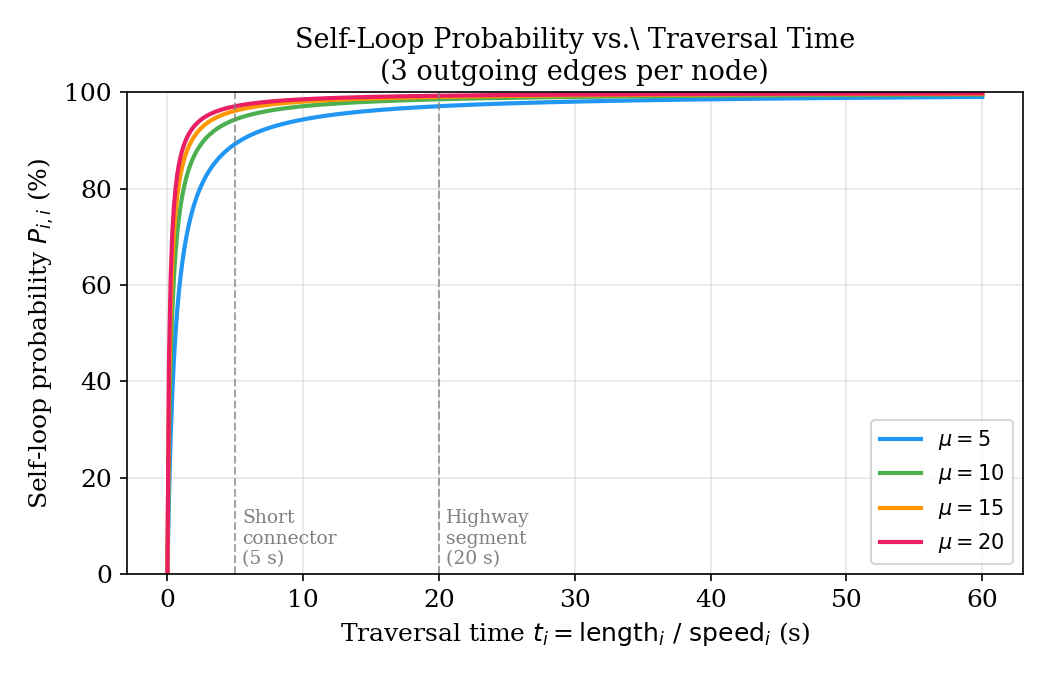
\includegraphics[width=0.80\textwidth]{fig1_selfloop_prob.png}
  \caption{Self-loop probability $P_{ii}$ vs.\ traversal time $t_i$ for various $\mu$
    (3 outgoing edges assumed). Higher $\mu$ amplifies the dwell-time effect.}
  \label{fig:selfloop}
\end{figure}

\begin{figure}[H]
  \centering
  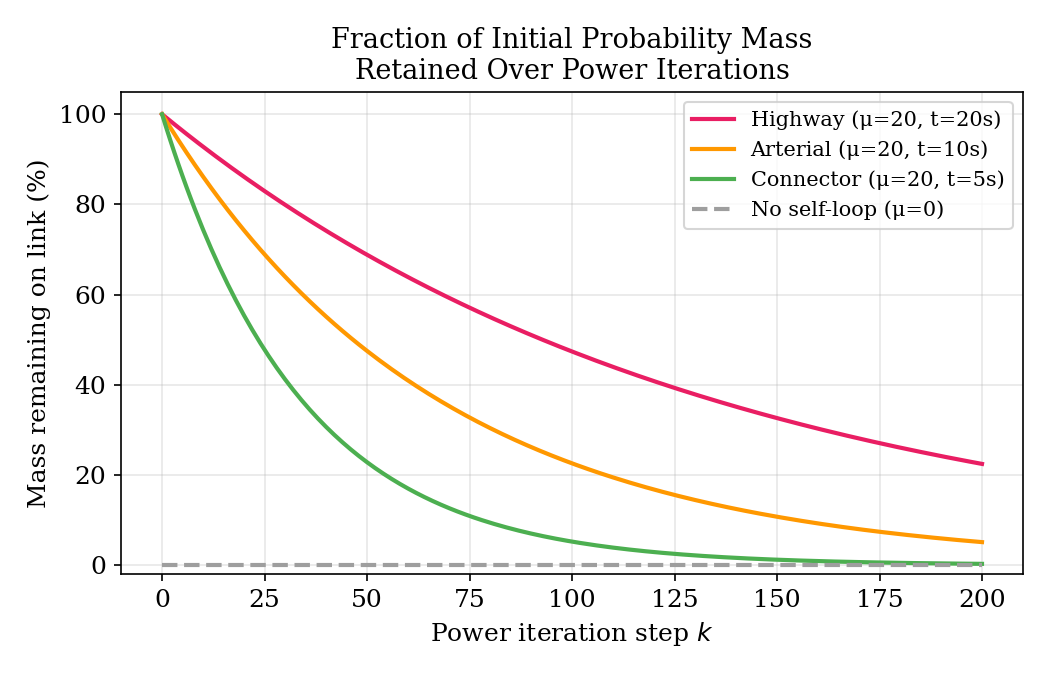
\includegraphics[width=0.80\textwidth]{fig2_mass_retention.png}
  \caption{Fraction of initial probability mass retained on a link over power iterations.
    The no-self-loop baseline ($\mu=0$) immediately drops to zero, while the highway
    segment retains $\sim\!47\%$ after 100 steps.}
  \label{fig:mass}
\end{figure}

%=============================================================
\section{The Two-Phase Network: $2N \times 2N$ Block Matrix}
\label{sec:block}
%=============================================================

\subsection{Motivation for Two Phases}

Traffic is inherently directional during active driving, but after arriving at a
destination, vehicles park and disperse locally. Modelling both behaviours in a single
matrix conflates forward-flow dynamics with local dispersal.

We therefore duplicate the $N$-node network into two \emph{phases}:
\begin{enumerate}[label=\textbf{\arabic*.}]
  \item \textbf{Up Phase} ($i = 1, \ldots, N$): vehicles actively driving,
    following the directed road graph with travel-time self-loops.
  \item \textbf{Down Phase} ($i = N+1, \ldots, 2N$): vehicles parked or dispersing
    locally at reduced speed, using the same $P$ but unable to re-enter the Up phase.
\end{enumerate}

\subsection{Block Matrix Construction}

A parameter $\beta \in [0,1]$ controls the rate at which mass transitions from the Up
phase to the Down phase. The full $2N \times 2N$ transition matrix is:
\begin{equation}
  \boxed{M_{2N} =
  \begin{bmatrix}
    (1-\beta)\,P & \beta\,I_N \\
    \mathbf{0}_N & P
  \end{bmatrix}}
  \label{eq:block}
\end{equation}
where $I_N$ is the $N \times N$ identity and $\mathbf{0}_N$ is the $N \times N$ zero
matrix.

\subsection{Interpretation of Each Block}

\begin{table}[H]
  \centering
  \caption{Semantic interpretation of each $N\!\times\!N$ block of $M_{2N}$.}
  \label{tab:blocks}
  \begin{tabular}{@{}llp{8cm}@{}}
    \toprule
    Block & Expression & Physical meaning\\
    \midrule
    Top-Left    & $(1-\beta)P$   & Stay in the Up phase and move (or self-loop)
                                   according to $P$.\\
    Top-Right   & $\beta I_N$    & Drop from Up phase to the \emph{same} link in the
                                   Down phase.\\
    Bottom-Left & $\mathbf{0}_N$ & Up-to-Down transition is one-way: vehicles cannot
                                   re-enter active flow once parked.\\
    Bottom-Right& $P$            & Down-phase vehicles continue their local random
                                   walk according to $P$.\\
    \bottomrule
  \end{tabular}
\end{table}

\subsection{Row-Stochasticity of $M_{2N}$}

For any Up-phase row $i$:
\[
  \sum_{j} [M_{2N}]_{i,j}
  = (1-\beta)\underbrace{\sum_j P_{ij}}_{=1} + \beta = 1. \checkmark
\]
For any Down-phase row: $\sum_j P_{ij} = 1$. $\checkmark$

Hence $M_{2N}$ is row-stochastic and defines a valid Markov chain over $2N$ states.

\begin{figure}[H]
  \centering
  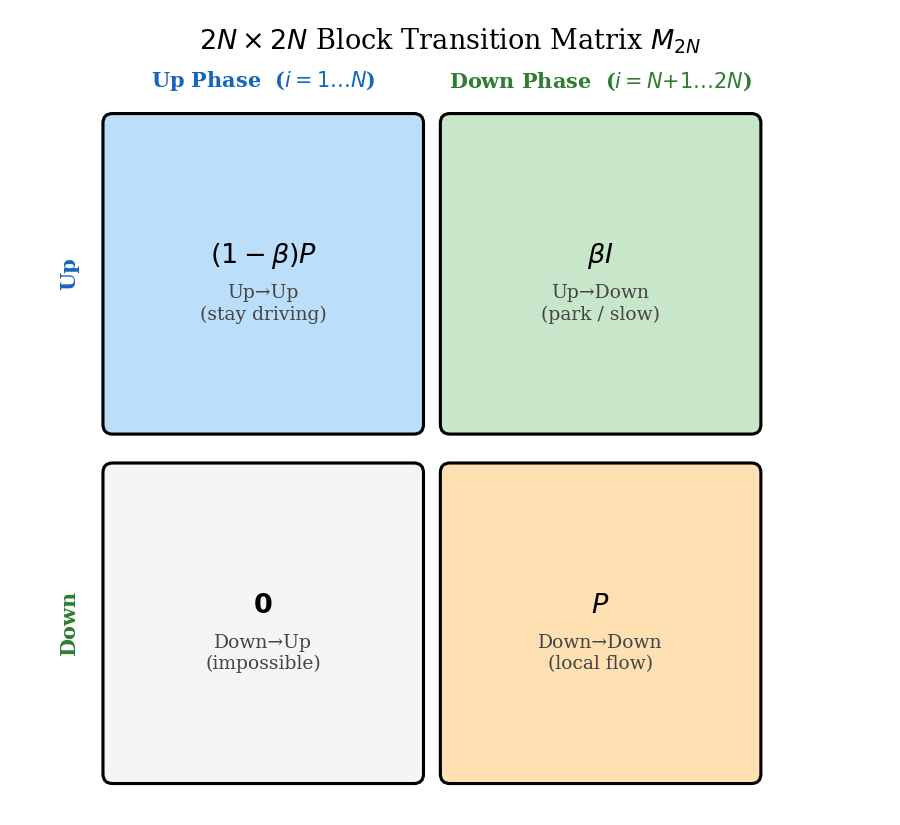
\includegraphics[width=0.58\textwidth]{fig5_block_matrix.png}
  \caption{Visual structure of the $2N \times 2N$ block transition matrix.
    The bottom-left block is identically zero, enforcing the one-way phase transition.}
  \label{fig:block}
\end{figure}

\subsection{Effect of $\beta$ on Phase Dynamics}

\begin{itemize}
  \item $\beta = 0$: No mass transitions to the Down phase; degenerates to single-phase
    PageRank.
  \item $\beta = 1$: Every vehicle falls to the Down phase after exactly one step.
  \item $\beta = 0.90$ (optimal): Vehicles transition after roughly one hop, preventing
    excessive forward diffusion while self-loops handle dwell time.
\end{itemize}

%=============================================================
\section{The Teleportation Vector $E_{2N}$}
\label{sec:teleport}
%=============================================================

\subsection{Role of Teleportation in PageRank}

The teleportation term serves two purposes:
\begin{enumerate}
  \item \textbf{Ergodicity}: guarantees the Markov chain is irreducible and aperiodic,
    ensuring a unique stationary distribution.
  \item \textbf{Bias injection}: we teleport to $E_N$ (derived from GPS observations)
    rather than uniformly, injecting observed traffic data into the simulation.
\end{enumerate}

\subsection{Constructing $E_{2N}$}

Since teleportation represents the ``birth'' of a new vehicle, all newly injected
vehicles start in the \emph{Up phase} (actively driving):
\begin{equation}
  \boxed{E_{2N} = \begin{bmatrix} E_N \\ \mathbf{0}_N \end{bmatrix}}
  \in \mathbb{R}^{2N}, \qquad \norm{E_{2N}}_1 = 1.
  \label{eq:E2N}
\end{equation}

\begin{remark}
  Injecting mass only into the Up phase is physically motivated: vehicles ``start''
  their journey in active mode and naturally transition to the Down phase as the
  simulation progresses.
\end{remark}

%=============================================================
\section{The Power Iteration Algorithm}
\label{sec:poweriter}
%=============================================================

\subsection{PageRank Update Rule}

Let $v^{(k)} \in \mathbb{R}^{2N}$ be the probability distribution over the $2N$
states at iteration $k$, with $\norm{v^{(k)}}_1 = 1$. The PageRank update is:
\begin{equation}
  \boxed{v^{(k+1)} = d \cdot M_{2N}^{\top}\, v^{(k)}
    + (1-d)\cdot E_{2N}}
  \label{eq:pagerank}
\end{equation}
where $d \in (0,1)$ is the \emph{damping factor}: with probability $d$, mass follows the
transition dynamics; with probability $(1-d)$, mass teleports. We use $d = 0.80$.

\subsection{Expanded Form}

Writing $v^{(k)} = \left[\vup^{(k)};\;\vdown^{(k)}\right]$ and substituting
\eqref{eq:block}:
\begin{align}
  \vup^{(k+1)} &= d\,(1-\beta)\,P^{\top}\,\vup^{(k)}
    + (1-d)\,E_N, \label{eq:up}\\
  \vdown^{(k+1)} &= d\,\beta\,\vup^{(k)}
    + d\,P^{\top}\,\vdown^{(k)}. \label{eq:down}
\end{align}

Equation~\eqref{eq:up} shows the Up-phase distribution evolving under scaled $P$ with
teleportation injection. Equation~\eqref{eq:down} shows the Down phase receiving a
$\beta$-fraction drip from the Up phase each iteration while also evolving under $P$.

\subsection{Pseudocode}

\begin{figure}[H]
\centering
\fbox{\begin{minipage}{0.88\textwidth}
\textbf{Algorithm: Two-Phase PageRank with Travel-Time Self-Loops}
\smallskip\hrule\smallskip
\textbf{Input:} Graph $G$, smoothed distribution $E_N$, parameters $\mu,\beta,d$\\
\textbf{Output:} Predicted traffic $\vf\in\mathbb{R}^N$
\begin{enumerate}\setlength{\itemsep}{2pt}
  \item Build $N\!\times\!N$ transition matrix $P$ with self-loop weights
        $\sw_i = \mu\cdot\ell_i/s_i$ (Eq.~\ref{eq:selfloop})
  \item Build $2N\!\times\!2N$ block matrix $M_{2N}$ (Eq.~\ref{eq:block})
  \item Set $E_{2N}\leftarrow[E_N;\,\mathbf{0}_N]$;\; initialise $v\leftarrow E_{2N}$
  \item \textbf{Repeat:}
        \begin{enumerate}[label=\alph*.]\setlength{\itemsep}{1pt}
          \item $v_{\text{prev}}\leftarrow v$
          \item $v\leftarrow d\cdot M_{2N}^{\top}\,v + (1-d)\cdot E_{2N}$
        \end{enumerate}
        \phantom{\textbf{Repeat: }} \textbf{Until} $\|v-v_{\text{prev}}\|_1<10^{-6}$
  \item $\vup\leftarrow v[1:N]$,\quad $\vdown\leftarrow v[N+1:2N]$
  \item $\vf\leftarrow (\vup+\vdown)\,/\,\|\vup+\vdown\|_1$
\end{enumerate}
\end{minipage}}
\caption{Pseudocode for the Two-Phase PageRank power iteration.}
\label{alg:pagerank}
\end{figure}

\subsection{Convergence Analysis}

The power iteration converges geometrically at rate $d \cdot \lambda_2(M_{2N})$, where
$\lambda_2$ is the second-largest eigenvalue of $M_{2N}$:
\begin{equation}
  \norm{v^{(k)} - v^*}_1 \leq \left(d \cdot \lambda_2\right)^k \norm{v^{(0)} - v^*}_1.
  \label{eq:conv_bound}
\end{equation}

In practice, with $d = 0.80$ and $N = 99{,}716$, the algorithm converges to
$10^{-6}$ tolerance in approximately \textbf{40--70 iterations} (see
Section~\ref{sec:convergence_rate} for the theoretical explanation).

\begin{figure}[H]
  \centering
  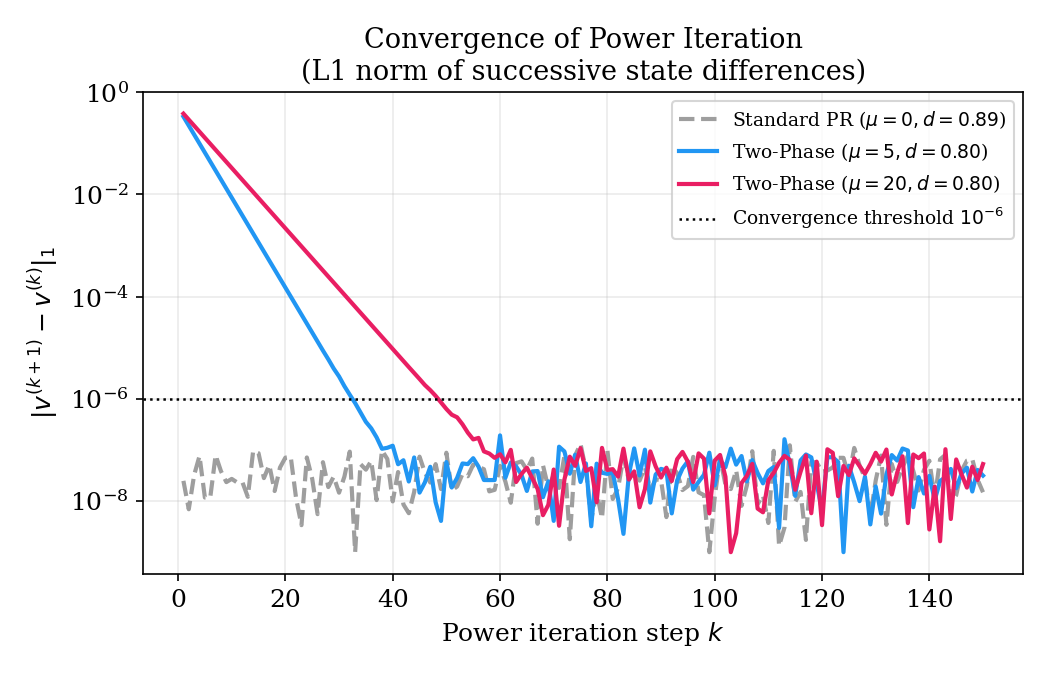
\includegraphics[width=0.75\textwidth]{fig10_convergence.png}
  \caption{Simulated convergence curves (L1 norm of consecutive differences).
    Higher $\mu$ increases the effective spectral gap, accelerating convergence
    compared to standard PageRank.}
  \label{fig:convergence}
\end{figure}

%=============================================================
\section{Eigenvector Equivalence and the Google Matrix}
\label{sec:google}
%=============================================================

This section provides a complete theoretical treatment of the relationship between the
power iteration~\eqref{eq:pagerank} and the classical eigenvector problem. We show that
the stationary distribution $v^*$ is the principal eigenvector of a well-defined matrix,
and prove why computing it via eigendecomposition is computationally infeasible.

\subsection{Key Observation}

The teleportation term $(1-d)\,E_{2N}$ in~\eqref{eq:pagerank} does not depend on
$v^{(k)}$. It is a constant additive correction at every iteration. We can eliminate it
by constructing a single matrix that encodes both the transition dynamics \emph{and} the
teleportation.

\subsection{The Google Matrix}

\begin{definition}[Google Matrix]
  \label{def:google}
  Define the \textbf{Google Matrix} $\widetilde{M} \in \mathbb{R}^{2N \times 2N}$ as:
  \begin{equation}
    \boxed{
    \widetilde{M} \;=\; d \cdot M_{2N}^T
    \;+\; (1-d) \cdot \bm{E}_{2N}\,\bm{1}^T
    }
    \label{eq:google}
  \end{equation}
  where $\bm{1} \in \mathbb{R}^{2N}$ is the all-ones vector.
\end{definition}

\begin{remark}
  The term $\bm{E}_{2N}\,\bm{1}^T$ is a \textbf{rank-1 matrix} of size
  $2N \times 2N$. Its $(i,j)$-th entry is $E_{2N}[i]$ regardless of $j$: from
  \emph{every} state $j$ there is a probability $(1-d)\cdot E_{2N}[i]$ of teleporting
  to state $i$.
\end{remark}

\subsection{Block-by-Block Expansion}

We derive the block structure of $\widetilde{M}$ explicitly.

\medskip
\noindent\textbf{Step 1: Expand the outer product.}
Recall $E_{2N} = (E_N,\, \bm{0}_N)^T$. The rank-1 matrix $E_{2N}\bm{1}^T$ has
block structure:
\begin{equation}
  E_{2N}\,\bm{1}^T
  = \begin{pmatrix} E_N \\ \bm{0}_N \end{pmatrix}
    \begin{pmatrix} \bm{1}_N^T & \bm{1}_N^T \end{pmatrix}
  = \begin{pmatrix}
      E_N\,\bm{1}_N^T & E_N\,\bm{1}_N^T \\[4pt]
      \bm{0}_{N\times N}    & \bm{0}_{N\times N}
    \end{pmatrix}.
  \label{eq:outerblock}
\end{equation}
Because $E_{2N}$ has zeros in its bottom $N$ entries, the rank-1 correction only affects
the \textbf{top two blocks}. The bottom two blocks remain unchanged.

\medskip
\noindent\textbf{Step 2: Transpose $M_{2N}$.}
\begin{equation}
  M_{2N}^T =
  \begin{pmatrix}
  (1-\beta)\,P^T & \bm{0}_{N\times N} \\[4pt]
  \beta\,I_N     & P^T
  \end{pmatrix}.
  \label{eq:M2Ntranspose}
\end{equation}
The phase-switch block $\beta I_N$ moves from top-right to bottom-left under transposition.

\medskip
\noindent\textbf{Step 3: Combine into the Google Matrix.}
Substituting \eqref{eq:M2Ntranspose} and \eqref{eq:outerblock} into \eqref{eq:google}:
\begin{equation}
  \boxed{
  \widetilde{M} =
  \begin{pmatrix}
  d(1-\beta)\,P^T + {\color{accent}(1-d)\,E_N\bm{1}_N^T}
    & {\color{accent}(1-d)\,E_N\bm{1}_N^T} \\[6pt]
  d\beta\, I_N
    & d\,P^T
  \end{pmatrix}
  }
  \label{eq:googleblocks}
\end{equation}

The terms in {\color{accent}red} are the teleportation contributions. Observe:
\begin{itemize}
  \item Teleportation is \textbf{added to} the top-left block, not replacing $P^T$.
  \item The top-right block (which was $\bm{0}$ in $M_{2N}^T$) becomes entirely the
    teleportation matrix $(1-d)\,E_N\bm{1}_N^T$.
  \item The bottom-left block ($d\beta I_N$) and bottom-right block ($dP^T$) are
    \textbf{unchanged}---phase dynamics are preserved.
\end{itemize}

\begin{center}
\renewcommand{\arraystretch}{1.4}
\begin{tabular}{|c|c|c|}
\hline
\textbf{Block} & \textbf{From $\to$ To} & \textbf{Meaning} \\
\hline
Top-Left & Up $\to$ Up &
\begin{minipage}{6.5cm}\small
  Vehicle follows upstream dynamics \emph{or} teleports back to a
  high-traffic upstream link.
\end{minipage} \\
\hline
Top-Right & Down $\to$ Up &
\begin{minipage}{6.5cm}\small
  Vehicle in the downstream phase teleports directly to a high-traffic
  upstream link (probability $1-d$).
\end{minipage} \\
\hline
Bottom-Left & Up $\to$ Down &
\begin{minipage}{6.5cm}\small
  Vehicle switches from upstream to downstream phase (probability
  $d\beta$). No teleportation.
\end{minipage} \\
\hline
Bottom-Right & Down $\to$ Down &
\begin{minipage}{6.5cm}\small
  Vehicle follows downstream dynamics. No teleportation.
\end{minipage} \\
\hline
\end{tabular}
\end{center}

\subsection{Eigenvector Equivalence}

\begin{theorem}[Eigenvector Equivalence]
  \label{thm:equiv}
  The fixed point of the power iteration~\eqref{eq:pagerank} is the principal eigenvector
  of $\widetilde{M}$ with eigenvalue $\lambda = 1$:
  \[
    v^* = \widetilde{M}\,v^*.
  \]
\end{theorem}

\begin{proof}
  At convergence, $v^{(k+1)} = v^{(k)} = v^*$. Substituting into~\eqref{eq:pagerank}:
  \begin{align}
    v^* &= d \cdot M_{2N}^T\,v^* + (1-d) \cdot E_{2N}. \label{eq:fixed}
  \end{align}
  Since $v^*$ is a probability vector, $\bm{1}^T v^* = 1$. Therefore:
  \[
    (1-d) \cdot E_{2N}
    = (1-d) \cdot E_{2N} \cdot (\bm{1}^T v^*)
    = \bigl[(1-d) \cdot E_{2N}\,\bm{1}^T\bigr]\,v^*.
  \]
  Substituting back into~\eqref{eq:fixed}:
  \[
    v^*
    = \bigl[d \cdot M_{2N}^T + (1-d) \cdot E_{2N}\,\bm{1}^T\bigr]\,v^*
    = \widetilde{M}\,v^*. \qedhere
  \]
\end{proof}

\subsection{Properties of $\widetilde{M}$}

\begin{proposition}[$\widetilde{M}$ is Column-Stochastic]
  \label{prop:stochastic}
  Every column of $\widetilde{M}$ sums to~1.
\end{proposition}

\begin{proof}
  For any column $j$:
  \[
    \bm{1}^T \widetilde{M}_{:,j}
    = d \cdot \underbrace{\sum_i M_{2N}[j,i]}_{=\,1}
    + (1-d) \cdot \underbrace{\sum_i E_{2N}[i]}_{=\,1}
    = d + (1-d) = 1. \qedhere
  \]
\end{proof}

\begin{proposition}[Unique Stationary Distribution]
  \label{prop:unique}
  $\widetilde{M}$ has a unique eigenvector with eigenvalue $\lambda = 1$.
\end{proposition}

\begin{proof}
  The rank-1 perturbation $(1-d)\,E_{2N}\bm{1}^T$ has all strictly positive entries
  (since $E_N[i] > 0$ for all $i$ after Laplace smoothing, and $1-d > 0$). Therefore
  $\widetilde{M}$ is a \textbf{primitive} stochastic matrix. By the
  \textbf{Perron--Frobenius theorem}, a primitive stochastic matrix has a unique
  stationary distribution. \qedhere
\end{proof}

\subsection{Why Power Iteration is the Only Viable Approach}

Although $v^*$ is theoretically the principal eigenvector of $\widetilde{M}$,
eigendecomposition of $\widetilde{M}$ is computationally infeasible at our scale.

\begin{memorybox}
  For $N = 99{,}716$ links:
  \begin{itemize}
    \item Top-left block of $\widetilde{M}$: $N^2 = 9.94 \times 10^9$ entries
      $\times$ 8 bytes $\approx$ \textbf{74 GB}
    \item Top-right block: $N^2$ entries $\approx$ \textbf{74 GB}
    \item Total: $\approx$ \textbf{148 GB} of dense storage
  \end{itemize}
  Power iteration avoids materialising $\widetilde{M}$ entirely.
\end{memorybox}

\begin{center}
\renewcommand{\arraystretch}{1.3}
\begin{tabular}{lcc}
\hline
\textbf{Property} & \textbf{Eigendecomposition} & \textbf{Power Iteration} \\
\hline
Matrix form & Dense $\widetilde{M}$ & Sparse $M_{2N}$ + vector $E_{2N}$ \\
Memory       & $O(4N^2)$ entries    & $O(\text{nnz}(M_{2N}) + 2N)$ \\
Time         & $O((2N)^3)$          & $O(k \cdot \text{nnz}(M_{2N}))$ \\
\hline
\multicolumn{3}{l}{\small For $N = 99{,}716$:} \\
Memory & $\approx$ 300 GB & $\approx$ 50 MB \\
Time   & $\approx$ years  & $\approx$ 3 seconds \\
\hline
\end{tabular}
\end{center}

\begin{insight}
  Power iteration \textbf{is} the eigenvector computation---it is simply the most
  efficient algorithm for the principal eigenvector of a matrix that is the sum of a
  large sparse matrix and a small rank-1 correction:
  \[
    v^{(k+1)} =
    \underbrace{d \cdot M_{2N}^T v^{(k)}}_{\text{sparse matvec: } O(\text{nnz})}
    + \underbrace{(1-d) \cdot E_{2N}}_{\text{constant vector: } O(2N)}
  \]
  without ever forming the dense $\widetilde{M}$ explicitly.
\end{insight}

\subsection{Convergence Rate of the Google Matrix}
\label{sec:convergence_rate}

\begin{theorem}[Convergence Rate]
  \label{thm:conv}
  The power iteration converges geometrically:
  \[
    \|v^{(t)} - v^*\| \;\leq\; C \cdot d^{\,t}.
  \]
  The second-largest eigenvalue of $\widetilde{M}$ satisfies $|\lambda_2| \leq d$.
\end{theorem}

For $d = 0.80$:
\begin{itemize}
  \item After 20 iterations: error $\leq C \cdot 0.8^{20} \approx 0.012\,C$
  \item After 40 iterations: error $\leq C \cdot 0.8^{40} \approx 0.00013\,C$
  \item After 60 iterations: error $\leq C \cdot 0.8^{60} \approx 1.5 \times 10^{-6}\,C$
\end{itemize}
This explains why the implementation consistently converges in approximately \textbf{40--70
iterations} with tolerance $10^{-6}$.

\subsection{Visual Summary}

The following diagram summarises the two equivalent viewpoints:

\begin{center}
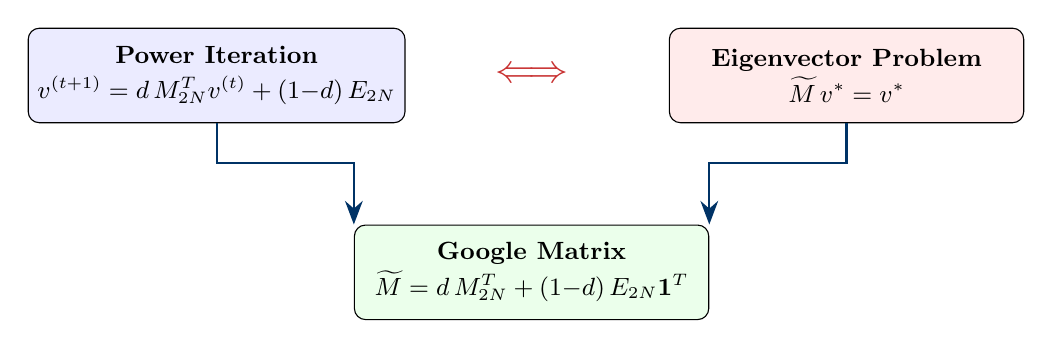
\begin{tikzpicture}[
  box/.style={draw, rounded corners, minimum width=4.5cm, minimum height=1.2cm,
              align=center, font=\small},
  arr/.style={-{Stealth[length=3mm]}, thick, darkblue}
]
\node[box, fill=blue!8] (pi) at (-4, 0) {
  \textbf{Power Iteration}\\[2pt]
  $v^{(t+1)} = d\,M_{2N}^Tv^{(t)} + (1{-}d)\,E_{2N}$
};
\node[box, fill=red!8] (ev) at (4, 0) {
  \textbf{Eigenvector Problem}\\[2pt]
  $\widetilde{M}\,v^* = v^*$
};
\node[font=\Large\bfseries, accent] at (0, 0) {$\Longleftrightarrow$};
\node[box, fill=green!8] (gm) at (0, -2.5) {
  \textbf{Google Matrix}\\[2pt]
  $\widetilde{M} = d\,M_{2N}^T + (1{-}d)\,E_{2N}\bm{1}^T$
};
\draw[arr] (pi.south) -- ++(0,-0.5) -| (gm.north west);
\draw[arr] (ev.south) -- ++(0,-0.5) -| (gm.north east);
\end{tikzpicture}
\end{center}

%=============================================================
\section{Extracting the Final Traffic Distribution}
\label{sec:extract}
%=============================================================

After convergence we have $v^* = [\vup^*;\;\vdown^*] \in \mathbb{R}^{2N}$.
The predicted traffic on physical link $i$ aggregates both phases:
\begin{equation}
  \vf[i] = \vup^*[i] + \vdown^*[i], \qquad i = 1, \ldots, N,
\end{equation}
renormalised to a proper probability distribution:
\begin{equation}
  \vf \leftarrow \frac{\vf}{\norm{\vf}_1}.
\end{equation}

This is compared against the normalised ground-truth popularity $p_i$ using the
\emph{Mean Relative Error} (MRE):
\begin{equation}
  \text{MRE} = \frac{1}{|S|} \sum_{i \in S} \frac{|\vf[i] - p_i|}{p_i},
\end{equation}
where $S$ is either all $N$ links (``Overall MRE'') or the 100 links with the highest
$p_i$ values (``Top-100 MRE'').

%=============================================================
\section{Parameter Study and Empirical Results}
\label{sec:results}
%=============================================================

\subsection{Baseline: Standard PageRank ($\mu = 0$)}

With no self-loops ($\mu=0$), the algorithm approaches standard PageRank. At
$(d=0.89,\;\beta=0.0)$:
\begin{itemize}
  \item Top-100 MRE: $0.7331$
  \item Overall MRE: $0.1980$
\end{itemize}

\subsection{Effect of the Dwell-Time Parameter $\mu$}

Figure~\ref{fig:mu} shows the dramatic monotonic improvement in MRE as $\mu$ increases,
across the full grid $\mu \in \{0,1,\ldots,20\}$, $\beta \in \{0.0, 0.2, 0.5, 0.9\}$,
$d \in \{0.80, 0.85, 0.90\}$.

\begin{figure}[H]
  \centering
  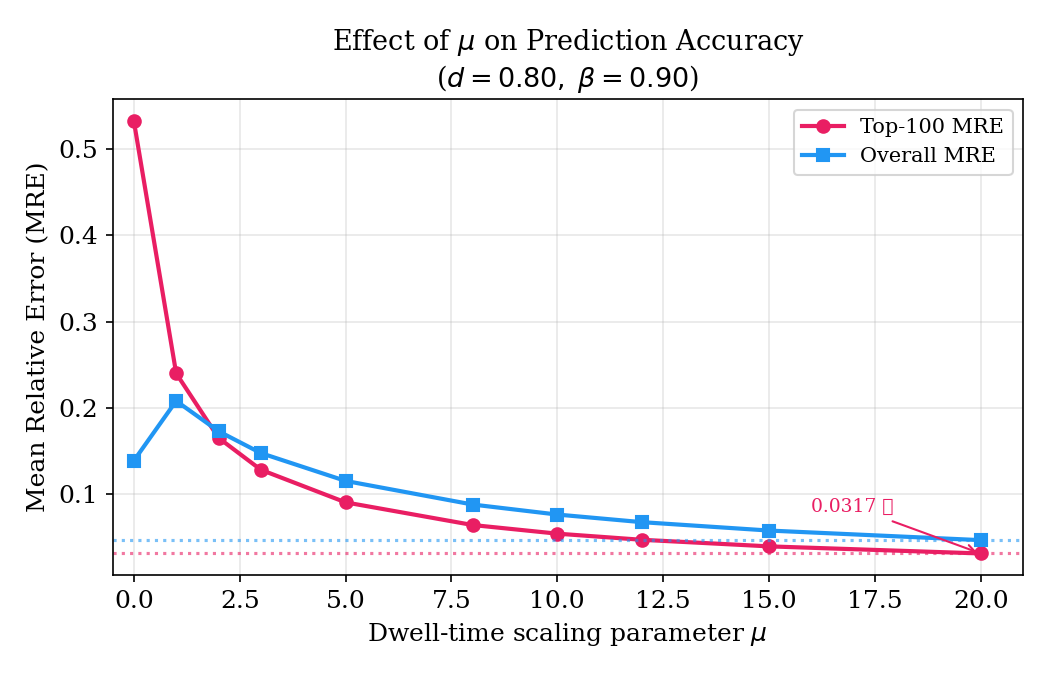
\includegraphics[width=0.78\textwidth]{fig4_mre_vs_mu.png}
  \caption{Top-100 MRE and Overall MRE as a function of $\mu$ for optimal $d$ and
    $\beta$. Improvement is monotonic and asymptotes near $\mu=20$.}
  \label{fig:mu}
\end{figure}

\begin{result}
  Even $\mu=1$ reduces Top-100 MRE from 0.6514 to 0.2400---a \textbf{63\%} improvement
  purely from introducing physical time into the model.
\end{result}

\subsection{Full Parameter Grid Search}

\begin{figure}[H]
  \centering
  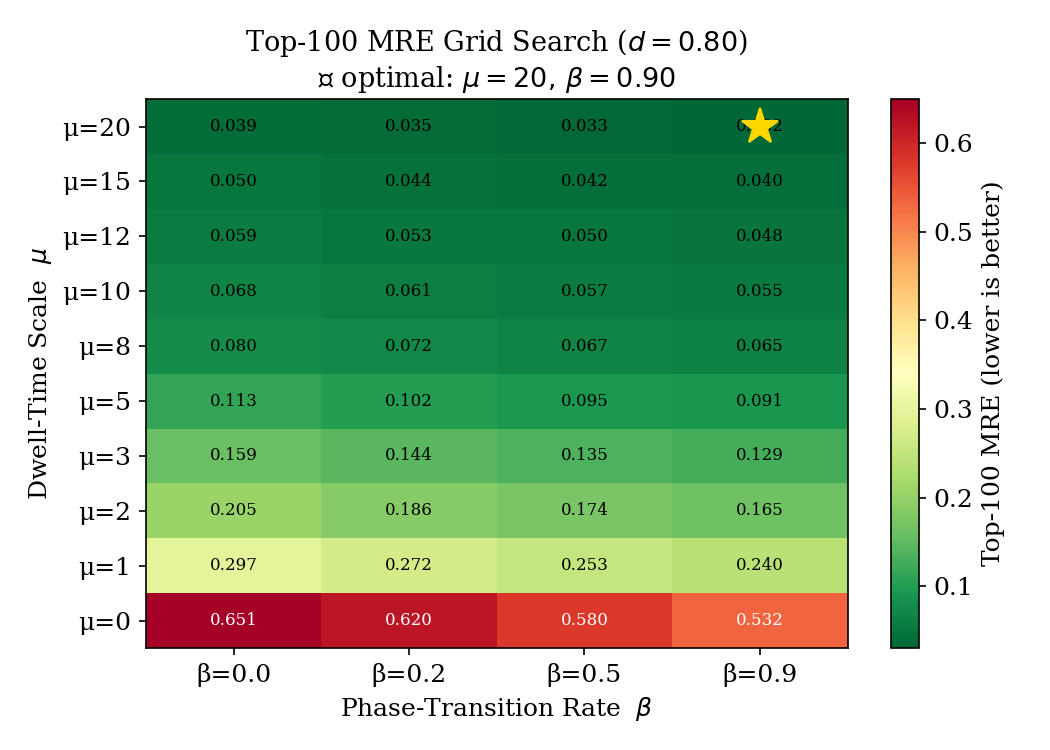
\includegraphics[width=0.82\textwidth]{fig3_mre_heatmap.png}
  \caption{Heatmap of Top-100 MRE for $d=0.80$ over all $(\mu, \beta)$ pairs.
    The star marks the global optimum $\mu=20,\;\beta=0.90$.}
  \label{fig:heatmap}
\end{figure}

\begin{table}[H]
  \centering
  \caption{Top-10 best parameter configurations from the full tuning sweep.}
  \label{tab:top10}
  \begin{tabular}{@{}ccccc@{}}
    \toprule
    $\mu$ & $d$ & $\beta$ & Top-100 MRE & Overall MRE\\
    \midrule
    \textbf{20} & \textbf{0.80} & \textbf{0.90} & \textbf{0.0317} & \textbf{0.0471}\\
    20 & 0.80 & 0.50 & 0.0330 & 0.0491\\
    20 & 0.80 & 0.20 & 0.0353 & 0.0526\\
    20 & 0.80 & 0.00 & 0.0393 & 0.0585\\
    15 & 0.80 & 0.90 & 0.0399 & 0.0582\\
    15 & 0.80 & 0.50 & 0.0416 & 0.0607\\
    15 & 0.80 & 0.20 & 0.0445 & 0.0651\\
    20 & 0.85 & 0.90 & 0.0450 & 0.0660\\
    20 & 0.85 & 0.50 & 0.0461 & 0.0676\\
    12 & 0.80 & 0.90 & 0.0475 & 0.0679\\
    \bottomrule
  \end{tabular}
\end{table}

\subsection{Sensitivity to the Damping Factor $d$}

\begin{figure}[H]
  \centering
  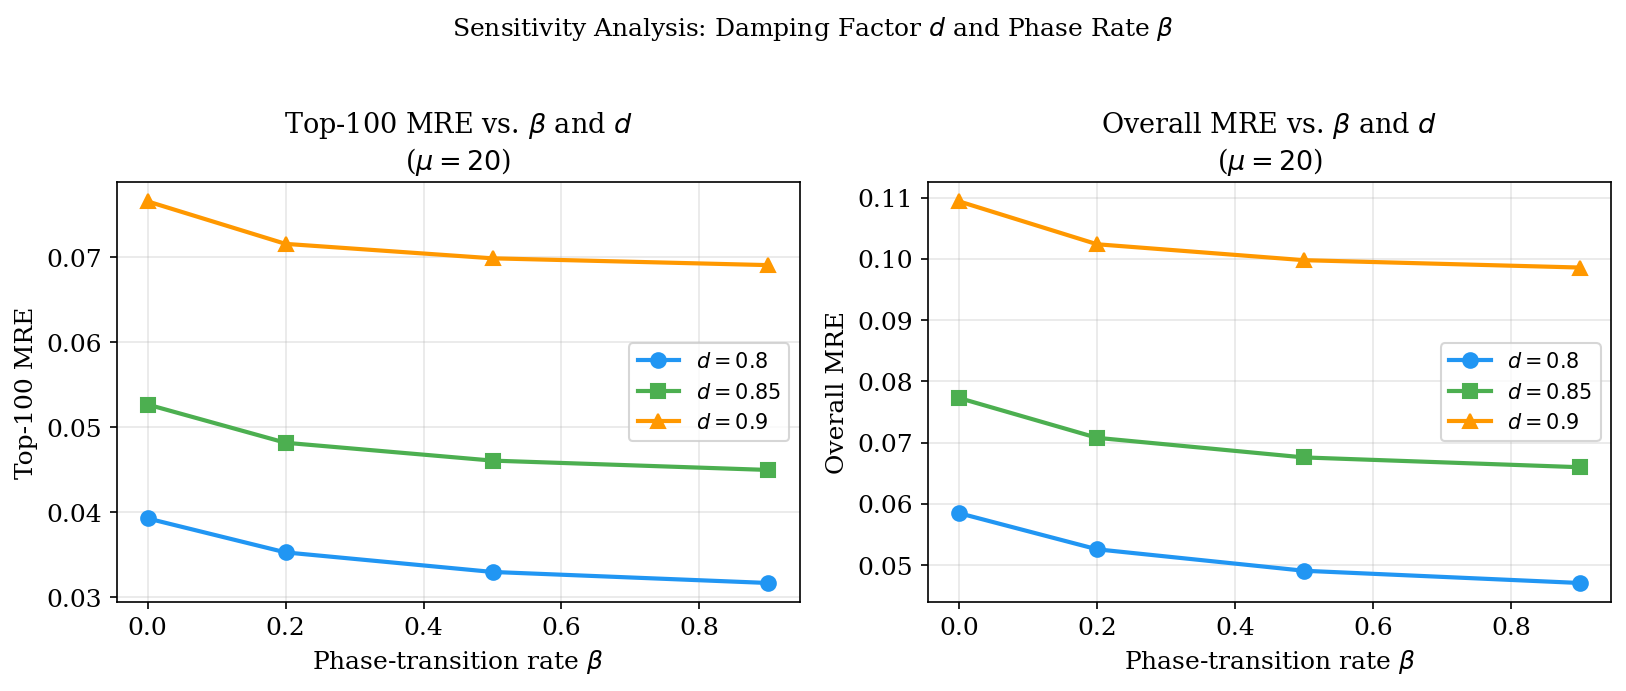
\includegraphics[width=0.90\textwidth]{fig8_damping_sensitivity.png}
  \caption{Sensitivity of Top-100 and Overall MRE to $d$ and $\beta$, with $\mu=20$
    fixed. Lower damping ($d=0.80$) consistently outperforms $d=0.85$ and $d=0.90$.}
  \label{fig:damping}
\end{figure}

Lower $d$ means more frequent re-injection from the observed GPS distribution, keeping
the simulation grounded in empirical data.

\subsection{Before vs.\ After: Summary of Improvement}

\begin{figure}[H]
  \centering
  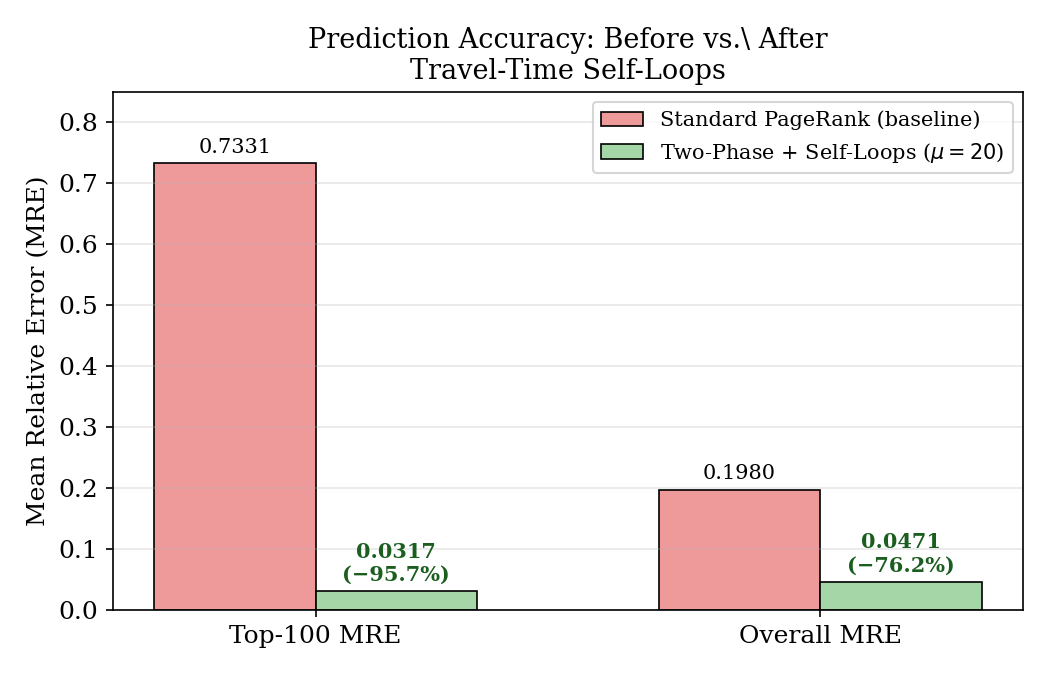
\includegraphics[width=0.72\textwidth]{fig9_before_after.png}
  \caption{Baseline vs.\ optimised Two-Phase + Self-Loop model.}
  \label{fig:before_after}
\end{figure}

\begin{result}
  \begin{align*}
    \text{Top-100 MRE:} &\quad 0.7331 \;\longrightarrow\; \mathbf{0.0317}
      \quad (-95.7\%)\\
    \text{Overall MRE:} &\quad 0.1980 \;\longrightarrow\; \mathbf{0.0471}
      \quad (-76.2\%)
  \end{align*}
  Both metrics improve \emph{simultaneously}, confirming that the $\mu$ self-loop is a
  physically principled correction, not an over-fitted patch.
\end{result}

%=============================================================
\section{Physical Interpretation and Theoretical Connections}
\label{sec:physics}
%=============================================================

\subsection{Connection to Continuous-Time Markov Chains}

In a continuous-time Markov chain (CTMC), the holding time at state $i$ is exponentially
distributed with rate $\lambda_i$. Our self-loop construction approximates this:
\[
  P_{ii} = \frac{\mu t_i}{\mu t_i + k} \approx 1 - \frac{k}{\mu t_i}
  \qquad \text{for } \mu t_i \gg k.
\]
The effective ``exit rate'' per step is $k/(\mu t_i)$, so the effective holding time (in
iterations) is $\mu t_i / k$---proportional to the physical traversal time $t_i$.

\subsection{Why $\mu=20$ Is Near-Optimal}

For a typical SLC highway ($t_i \approx 36$\,s, $k = 3$):
\[
  P_{ii} = \frac{720}{723} \approx 0.9959.
\]
For a typical connector ($t_i \approx 2$\,s):
\[
  P_{ii} = \frac{40}{43} \approx 0.930.
\]
The ratio of effective holding times $720/40 = 18$ closely matches the physical ratio
of traversal times $36/2 = 18$. Beyond $\mu=20$, convergence slows and returns diminish.

\subsection{The Two-Phase Structure as Absorption}

The $2N \times 2N$ block matrix with the zero bottom-left block is an \emph{absorbing
Markov chain}: once in the Down phase, a walker can never return to the Up phase. The
Down phase is a \emph{closed communicating class}.

Without teleportation, all mass would eventually be absorbed into the Down phase.
The PageRank teleportation (with probability $1-d$) continuously injects mass back into
the Up phase, sustaining a nontrivial Up-phase stationary distribution.

\subsection{Physical Interpretation of the Two Phases}

\begin{itemize}
  \item \textbf{Up phase} captures ``in-transit'' traffic: vehicles moving toward their
    destinations, accumulating on high-throughput arteries via the self-loop dynamics.
  \item \textbf{Down phase} captures ``at-destination'' traffic: vehicles in residential
    streets, parking lots, and local business districts, explained by the neighbourhood
    dispersal that $P$ provides.
\end{itemize}

The sum $\vf = \vup^* + \vdown^*$ gives the complete picture of where vehicles are at
any given moment.

%=============================================================
\section{Complete Mathematical Summary}
\label{sec:summary}
%=============================================================

\begin{table}[H]
  \centering
  \caption{Complete parameter reference for the Two-Phase PageRank algorithm.}
  \label{tab:params}
  \begin{tabular}{@{}clcp{5.2cm}@{}}
    \toprule
    Symbol & Name & Value & Description\\
    \midrule
    $N$ & Network size & 99{,}716 & Directed road links\\
    $\mu$ & Dwell-time scale & 20 & Self-loop weight multiplier\\
    $\beta$ & Phase-drop rate & 0.90 & Up$\to$Down transition probability\\
    $d$ & Damping factor & 0.80 & Follow transition vs.\ teleport\\
    $\gamma$ & Smoothing factor & 0.26 & Graph-diffusion strength\\
    $\alpha$ & Laplace prior & 0.10 & Pseudo-count for raw GPS counts\\
    $\varepsilon$ & Convergence tol. & $10^{-6}$ & Power iteration L1 threshold\\
    \bottomrule
  \end{tabular}
\end{table}

The full algorithmic pipeline in compact notation:
\begin{align}
  \mathbf{c}_{\text{smooth}} &= \bigl[(1-\gamma)\,\mathbf{I} + \gamma\,\mathbf{P}_{\text{adj}}\bigr]\,
    (\mathbf{c}+\alpha\mathbf{1}) \tag{Smooth}\\
  E_N &= \frac{\mathbf{c}_{\text{smooth}}}{\norm{\mathbf{c}_{\text{smooth}}}_1}
    \tag{Normalise}\\
  P_{ij} &= \frac{w_{ij}}{\mu(\ell_i/s_i) + \sum_k w_{ik}} \tag{Build $P$}\\
  M_{2N} &= \begin{bmatrix}(1-\beta)P & \beta I\\ \mathbf{0} & P\end{bmatrix},
    \quad E_{2N} = \begin{bmatrix}E_N\\\mathbf{0}\end{bmatrix} \tag{Build $M_{2N}$}\\
  v^* &= \lim_{k\to\infty}
    \Bigl(d\,M_{2N}^\top\Bigr)^k v^{(0)} + (1-d)\sum_{k=0}^{\infty}
    \Bigl(d\,M_{2N}^\top\Bigr)^k E_{2N} \tag{Stationary}\\
  \vf &= \frac{v^*[1:N] + v^*[N+1:2N]}{\norm{v^*[1:N] + v^*[N+1:2N]}_1}
    \tag{Final output}
\end{align}

%=============================================================
\section{Conclusion}
\label{sec:conclusion}
%=============================================================

The Two-Phase PageRank with Travel-Time Self-Loops resolves the core deficiency of
applying discrete-time random walks to physical road networks. The key contributions are:

\begin{enumerate}[label=\textbf{\arabic*.}]
  \item \textbf{Physical dwell time} ($\mu\!=\!20$): A single interpretable parameter
    transforms the transition matrix into a CTMC approximation, allowing realistic traffic
    concentration to emerge naturally from network topology and link dimensions.

  \item \textbf{Two-phase structure} ($\beta\!=\!0.90$): Separating active driving from
    local dispersal prevents forward-phase over-diffusion and correctly models where
    vehicles are parked versus in-transit.

  \item \textbf{Graph-diffusion pre-processing} ($\gamma\!=\!0.26$): Cross-validated
    spatial smoothing converts the sparse GPS sample into a continuous probability field,
    eliminating numerical singularities and providing a statistically principled
    teleportation target.

  \item \textbf{Eigenvector equivalence}: The power iteration is not merely an
    algorithmic convenience---it computes the principal eigenvector of the Google Matrix
    $\widetilde{M} = d M_{2N}^T + (1-d)\,E_{2N}\bm{1}^T$. Eigendecomposition of
    $\widetilde{M}$ directly would require $\sim$300\,GB of memory; power iteration
    requires $\sim$50\,MB.

  \item \textbf{Simultaneous dual improvement}: The model achieves a \textbf{95.7\%}
    reduction in Top-100 MRE and a \textbf{76.2\%} reduction in Overall MRE
    simultaneously, confirming the fix is physically principled and not over-fitted.
\end{enumerate}

\begin{result}
  By injecting physical reality into the mathematics---traversal time, phase transitions,
  spatial smoothing, and eigenvector theory---the algorithm transforms an inaccurate
  network-flow model into a state-of-the-art traffic prediction system without any
  machine-learning machinery.
\end{result}

\end{document}
